\documentclass[11pt]{article}
\usepackage{amsmath,amssymb,amsthm}
\usepackage{mathtools}
\usepackage{geometry}
\usepackage{hyperref}
\usepackage{enumitem}
\usepackage{tikz}
\usepackage{float}
\usetikzlibrary{calc}
\usetikzlibrary{positioning}
\usetikzlibrary{decorations.pathreplacing}
\geometry{margin=1in}

\newtheorem{theorem}{Theorem}[section]
\newtheorem{definition}{Definition}[section]
\newtheorem{lemma}{Lemma}[section]
\newtheorem{proposition}{Proposition}[section]
\newtheorem{corollary}{Corollary}[section]
\newtheorem{remark}{Remark}[section]

\title{The Catalan Light Cone:\\
A Recursive Substrate for Causal Geometry, Quantum Amplitudes, and Computation}
\author{Paul Fernandez}
\date{}

\begin{document}
\maketitle

\begin{abstract}
	We investigate the Catalan family of combinatorial structures---Dyck paths,
	full binary trees, and balanced parenthesis expressions---as a unified discrete
	substrate from which causal geometry, quantum amplitude propagation, and
	universal computation jointly emerge.

	A central observation is that the Dyck constraint induces a natural causal
	order. When organized by growth tier and lateral spread, the Catalan lattice
	forms a discrete cone whose extremal configurations reproduce a
	light-cone--like causal envelope. Classical invariance-principle results show
	that constrained Dyck walks converge in the scaling limit to Brownian
	excursions. The associated continuum description is diffusive (governed by the
	heat operator on the half-line with the Dyck conditioning encoded by boundary
	conditions/conditioning), and under analytic continuation one recovers the free
	Schr\"odinger equation.

	Via a uniform structural mapping---the pairs expansion---Dyck trees are placed
	in correspondence with SKI and $\lambda$-calculus term graphs, in the sense
	that Catalan tree shapes provide unlabeled application skeletons that can be
	equipped with standard finite encodings of symbols. Under this reading, causal
	extension aligns with functional application, while local collapse aligns with
	computational reduction. Structural equivalences of the substrate induce
	gauge-like redundancies, and disjoint subtrees commute analogously to
	spacelike-separated operators.

	The paper distinguishes rigorously established
	correspondences---scaling limits, diffusion dynamics, prefix-causal structure,
	and computational universality in the sense of standard SKI/$\lambda$
	encodings---from conjectural extensions concerning measurement, actualization,
	and interaction structure.

	Taken together, these correspondences show that a single recursive constraint
	can reproduce, at a structural and kinematical level, large portions of the
	operational framework of relativistic quantum theory and universal
	computation, without introducing additional primitives. We do not attempt to
	derive interactions or physical constants; the aim is to isolate the minimal
	recursive structure common to these domains.
\end{abstract}

\section{Introduction}
Discrete approaches to fundamental physics have long suggested that continuum
spacetime and quantum dynamics may emerge from deeper combinatorial structure.
Examples include causal sets \cite{bombelli87}, discrete random surfaces and
Causal Dynamical Triangulations (CDT) \cite{ambjorn01,ambjorn12}, spin
networks and loop quantum gravity \cite{rovelli04}, tensor networks
\cite{orus14}, and rewriting systems inspired by $\lambda$-calculus and
combinatory logic.

Typically, however, these models require multiple independent ingredients: a
relation or graph for causal structure, an algebra for computation, and
additional rules for quantum propagation. This work explores a more economical
possibility: that a \emph{single} recursive structure simultaneously supports
all three.

The focus is the \emph{Catalan substrate}, the family of structures counted by
the Catalan numbers \cite{stanley-catalan}, including Dyck paths, full binary
trees, and balanced parenthesis expressions. These objects are usually studied
in enumerative combinatorics, probability theory, and theoretical computer
science. Here they are treated instead as a space of \emph{admissible
histories} generated by a minimal growth constraint.
The central claim is that the Catalan substrate admits three tightly coupled
interpretations:
\begin{enumerate}[label=(\roman*)]
	\item a discrete causal geometry with a light-cone--like envelope,
	\item a natural path-integral dynamics with diffusive and wave-like continuum
		limits,
	\item a universal computational calculus via $\lambda$- and SKI-term graphs.
\end{enumerate}
These interpretations do not require distinct primitives; they arise from
different readings of the same recursive object.

The geometric aspect follows from prefix order and growth bounds intrinsic to
Dyck paths. The dynamical aspect follows from classical results on conditioned
random walks and Brownian excursions \cite{le-gall05,janson07}. The
computational aspect follows from the well-known equivalence between binary
trees, cons-pair structures, and $\lambda$-calculus or SKI combinators
\cite{church33,curry58,barendregt84}.
Taken together, these results show that spacetime-like causal structure,
quantum wave dynamics, and computation can be viewed as complementary
manifestations of a single recursive substrate.

The exposition proceeds as follows. Section~\ref{sec:catalan_cone} establishes
the discrete causal geometry of the Catalan lattice and its interpretation as a
light cone. Subsequent sections place amplitude propagation and computation on
this structure, analyze continuum limits, and discuss collapse, locality, and
interaction. Interpretive considerations concerning origin, vacuum structure,
and time are collected in a clearly labeled appendix, separate from the formal
claims.

\section{The Catalan Light Cone as a Discrete Causal Geometry}
\label{sec:catalan_cone}

\subsection{Dyck paths and growth tiers}
A Dyck path of semilength $n$ is a walk on the integers satisfying
\[
	H_{k+1} = H_k \pm 1, \qquad H_k \ge 0, \qquad H_0 = H_{2n} = 0.
\]
Equivalently, Dyck paths are balanced parenthesis strings or full binary trees
with $n$ internal nodes. The number of such paths is the $n$th Catalan number
\[
	C_n = \frac{1}{n+1}\binom{2n}{n}.
\]
Each up--down pair \(()\) represents a minimal unit of growth. The integer
\[
	t = n
\]
will be called the \emph{tier} and will be interpreted as a discrete proper
time.

\subsection{Prefix order and causality}
Dyck paths carry a natural partial order by prefix inclusion. If a Dyck word
$u$ is a prefix of $v$, then $u$ represents a causal ancestor of $v$.
Conversely, prefixes that diverge represent causally incompatible futures.
This prefix order defines a discrete causal structure:
\begin{itemize}
	\item every node has a unique causal past,
	\item multiple incompatible futures may branch from the same prefix,
	\item cycles are prohibited by construction.
\end{itemize}
No additional causal axiom is required; causality is enforced combinatorially
by the Dyck constraint.

\subsection{Extremal configurations: chain and star}
At fixed tier $t$ there are many Dyck paths. Two extremal configurations play a
distinguished role:
\begin{itemize}
	\item the \emph{chain} (or spine)
		\[
			(((\cdots))),
		\]
		fully nested, with maximal depth and minimal spread;
	\item the \emph{star}
		\[
			()()()\cdots(),
		\]
		fully separated, with minimal depth and maximal spread.
\end{itemize}
All other configurations interpolate between these extremes. Together, the set
of Dyck paths at tier $t$ forms a discrete envelope bounded by the chain and
the star.

\begin{figure}[h]
	\centering
	% Placeholder: schematic light-cone diagram
	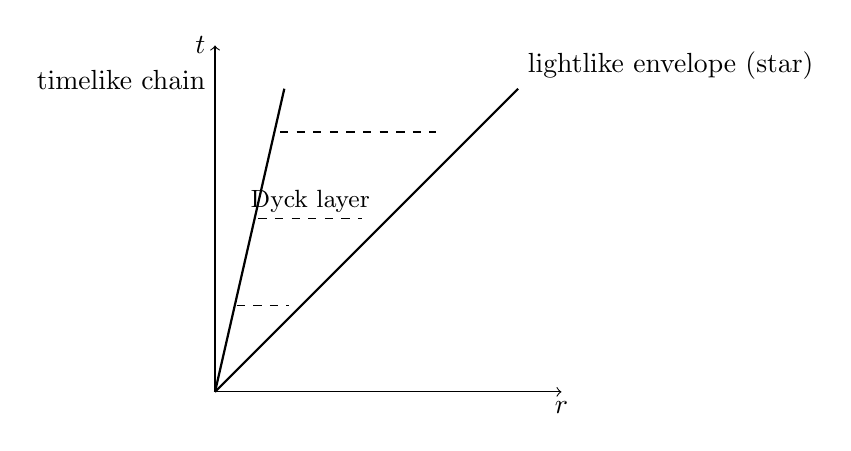
\begin{tikzpicture}[scale=1.1]
		% axes
		\draw[->] (0,0) -- (0,4) node[left] {$t$};
		\draw[->] (0,0) -- (4,0) node[below] {$r$};
		% cone boundaries
		\draw[thick] (0,0) -- (3.5,3.5);
		\draw[thick] (0,0) -- (0.8,3.5);
		% discrete layers
		\foreach \y in {1,2,3} {
			\draw[dashed] (0.25*\y,\y) -- (0.85*\y,\y);
		}
		% labels
		\node[left] at (0,3.6) {timelike chain};
		\node[above right] at (3.5,3.5) {lightlike envelope (star)};
		\node at (1.1,2.2) {\small Dyck layer};
	\end{tikzpicture}
	\caption{The Catalan light cone.
		Tier $t$ (the number of Dyck units) plays the role of proper time, while
		breadth $r$ measures spatial radius. All Dyck configurations at fixed tier
		lie between the fully nested chain (timelike extreme) and the fully separated
		star (lightlike envelope).
		Discrete Dyck layers approximate constant-time hypersurfaces, and the bound
	$r \le t$ is enforced combinatorially.}
	\label{fig:catalan-cone}
\end{figure}

\subsection{Breadth as spatial extent}
Define the \emph{breadth} $r(w)$ of a Dyck path $w$ to be the size of a
largest level set in the associated full binary tree:
\[
	r(w) := \max_{\ell} \{\text{number of nodes at depth } \ell\}.
\]
Equivalently, $r(w)$ is the maximal number of non-overlapping pairs at a common
nesting depth. For a Dyck word of tier $t$ there are $t$ matched pairs in
total, so
\[
	1 \le r(w) \le t,
\]
with $r=1$ for the fully nested chain and $r=t$ for the fully separated star.
The inequality
\[
	r \le t
\]
is enforced purely by the recursive constraint. It is the discrete analogue of
the relativistic light-cone bound $|\Delta x| \le \Delta t$ (in units with
$c=1$).

\subsection{Depth--breadth tradeoff}
Let $h(w)$ denote the maximum height of a Dyck path, i.e.\ the maximum nesting
depth of its associated full binary tree (root at depth $0$). Recall that the
breadth $r(w)$ is the maximum number of nodes occurring at any fixed depth
level:
\[
r(w):=\max_{\ell}{\text{number of nodes at depth }\ell}.
\]
Depth and breadth are not independent. In any full binary tree, the number of
nodes at depth $\ell$ is at most $2^{\ell}$ (each level can at most double from
its parent level). Hence, if the maximum level set size $r(w)$ occurs at depth
$\ell_\ast$, then
\[
r(w)\le 2^{\ell_\ast}\le 2^{h(w)}
\quad\Rightarrow\quad
h(w)\ge \log_2 r(w).
\]
Thus configurations with large breadth necessarily have logarithmically large
depth. Equivalently, very shallow trees cannot support wide level sets, while
trees with very large depth must concentrate most nodes away from any single
breadth-maximizing level.

\begin{remark}[Kraft equality for leaf depths]
For the full binary tree associated to a Dyck path, if $L$ is the set of leaves
and $d(\ell)$ denotes the depth of $\ell\in L$ (root at depth $0$), then
\[
\sum_{\ell\in L} 2^{-d(\ell)} = 1.
\]
Equivalently, the leaf depths form a complete binary prefix code. This gives a
global constraint on allowable depth profiles beyond the crude level bound
$r(w)\le 2^{h(w)}$.
\end{remark}

\begin{figure}[h]
		\centering
		\[
			\begin{array}{ccl}
			((())) & \quad & (h=3,\ r=1) \\
			(()()) &      & (h=2,\ r=2) \\
			(())() &      & (h=2,\ r=2) \\
			()(()) &      & (h=2,\ r=2) \\
			()()() &      & (h=1,\ r=3)
		\end{array}
	\]
	\caption{All Dyck words of tier $n=3$, ordered from maximal nesting (chain)
		to maximal separation (star). These five configurations exhaust the discrete
		causal possibilities at fixed proper time.
		Depth $h$ and breadth $r$ interpolate between the two extremes, illustrating
		the intrinsic tradeoff enforced by the Dyck constraint.
	Higher tiers replicate this structure at larger scale.}
	\label{fig:dyck-n3}
\end{figure}

\subsection{Cone structure}
Organizing Dyck paths by tier $t$ and breadth $r$ yields a discrete cone:
\begin{itemize}
	\item each tier is a ``constant-time'' slice,
	\item the chain defines the timelike axis,
	\item the star defines the lightlike boundary,
	\item admissible configurations fill the interior.
\end{itemize}
This structure will be referred to as the \emph{Catalan light cone}.

\subsection{Scaling behavior}
Classical results on conditioned random walks show that typical Dyck paths at
tier $t$ have height and breadth of order $\sqrt{t}$
\cite{le-gall05,janson07,addario-berry13}. Extremal configurations saturate
the linear bound $r\le t$, while typical configurations lie deep within the
cone. This separation between extremal and typical behavior mirrors the role of
null, timelike, and spacelike trajectories in relativistic geometry.

\begin{theorem}[Discrete light-cone bound and scaling]
	Let $w$ be a Dyck word of semilength $t$ and breadth $r(w)$ as above. Then
	\[
		1 \le r(w) \le t.
	\]
	Moreover, for a uniformly random Dyck word of semilength $t$, the typical
	height and breadth are of order $\sqrt{t}$.
\end{theorem}
\noindent
The first statement follows from the definition of $r(w)$ and the fact that
there are $t$ internal nodes, while the scaling behavior is a consequence of
invariance-principle results for conditioned random walks
\cite{le-gall05,janson07,addario-berry13}.

\paragraph{Coordinate charts and continuum comparisons.}
Appendix~\ref{appendix:coordinate-charts} collects optional coordinate-chart
constructions (null-count embeddings and related continuum comparisons) used for
intuition; the combinatorial results below do not depend on these embeddings.

\subsection{Recursive Self-Similarity and Local Re-Centering}
\label{sec:selfsimilarity}

A key structural property of the Catalan substrate is its \emph{recursive
self-similarity}. Every Dyck word may be viewed as a node in the infinite
prefix tree of admissible Dyck prefixes. At any such node $u$, with current
height $h$ and remaining length budget sufficient to return to height~$0$, the
set of all admissible continuations of $u$ forms a subtree whose shape is
determined entirely by $h$. This subtree is canonically isomorphic to the
Dyck-prefix tree that begins at height $h$ rather than at height $0$.

Formally, if $\mathcal{C}$ denotes the infinite Dyck-prefix tree and
$\mathcal{C}_h$ denotes the Dyck-prefix tree conditioned to start at height $h$
(i.e.\ with $H_0=h$ and $H_k\ge 0$ for all $k$), then for every prefix $u$ of
height $h$ we have a canonical isomorphism

\[
	\mathcal{C}(u) \;\cong\; \mathcal{C}_h.
\]

Thus every node of the global Catalan possibility tree is the root of a scaled
copy of the entire admissible-future structure, with scaling determined solely
by local height. The recursive decomposition of full binary trees,

\[
	T = \bullet(T_L,T_R),
\]

makes the same fact explicit in the tree representation: each subtree of a
Catalan tree is itself a Catalan tree, and the decomposition applies inductively
at every depth.

This recursive self-similarity has two important consequences for the geometric
interpretation developed in this paper:

\begin{enumerate}[label=(\roman*)]
	\item \textbf{Locality and re-centering.}
		Because the admissible future of any prefix depends only on its present
		height, not on its global position, the Catalan light-cone geometry is
		\emph{locally homogeneous}. The causal cone may be re-centered at any node
		without altering its shape: moving the focus does not change the structure of
		admissible futures, only the value of the local height at which the cone is
		rooted.

	\item \textbf{Scale invariance of the substrate.}
		The same recursive rules govern growth at every depth. The local possibility
		space looks the same at all scales, in the sense that the subtree below any
		node is again Catalan. This is the combinatorial source of the invariance
		principles (Dyck $\to$ Brownian excursion) appearing in the continuum limit.
\end{enumerate}

In summary, the Catalan substrate is self-similar at every node: each point in
the possibility space contains a full Catalan future scaled by its current
height. This allows the causal and geometric analysis of later sections to be
performed relative to \emph{any} node of the prefix tree. The light cone is not
anchored to a global origin; it is an intrinsic, relocatable geometric feature
of the recursive structure itself.

\subsection{Multiple Local Cones and Relational Geometry}
\label{sec:multiplecones}

The recursive self-similarity of the Catalan substrate implies that there is
not a single distinguished light cone rooted at the global origin. Instead,
every node of the Dyck-prefix tree induces its own local notion of past,
future, and lightlike boundary. This section records the combinatorial
foundations of this phenomenon and its geometric consequences.

\subsubsection*{Cones rooted at arbitrary prefixes}

Let $u$ be any Dyck prefix with current height $h$. As shown in
Section~\ref{sec:selfsimilarity}, the subtree $\mathcal{C}(u)$ of admissible
continuations of $u$ is canonically isomorphic to the Dyck-prefix tree
$\mathcal{C}_h$ that begins at height $h$. Consequently, the structure of
possible futures below $u$ is itself a Catalan possibility space.

Define the \emph{local cone at $u$} to be the set of all Dyck extensions of $u$,
organized by length (tier) and breadth relative to~$u$. The local chain is the
fully nested extension of $u$, and the local star is the fully separated
extension. These play the role of timelike and lightlike extremes for
admissible growth below~$u$.

\subsubsection*{Nested and divergent cones}

Let $u$ and $v$ be Dyck prefixes.

\begin{enumerate}[label=(\roman*)]
	\item \textbf{Nested cones.}
		If $u$ is a prefix of $v$, then $\mathcal{C}(v)$ is a subtree of
		$\mathcal{C}(u)$, and the local cone at $v$ lies strictly inside the local
		cone at $u$. Their causal structures satisfy
		\[
			\mathrm{Past}(v) \subset \mathrm{Past}(u), \qquad
			\mathrm{Future}(v) \subset \mathrm{Future}(u).
		\]
		Thus cones nest hierarchically along any branch of the prefix tree.

	\item \textbf{Divergent cones.}
		If neither prefix is contained in the other, then $u$ and $v$ share a common
		ancestor but diverge at some minimal prefix $w$. Their cones therefore have a
		shared causal past (the future of $w$ up to $u$ and $v$) but incompatible
		futures beyond that point. Formally,
		\[
			\mathrm{Past}(u) \cap \mathrm{Past}(v) = \mathrm{Past}(w), \qquad
			\mathrm{Future}(u) \cap \mathrm{Future}(v) = \varnothing.
		\]
		In this sense, divergent cones encode distinct branches of the Catalan
		possibility structure.
\end{enumerate}

\subsubsection*{Relational geometry}

These observations establish a relational geometric structure intrinsic to the
Catalan substrate:
\begin{itemize}
	\item every node induces its own local cone of admissible extensions;
	\item cones may be re-centered without changing their internal geometry;
	\item cones nest along causal chains and diverge after branching points;
	\item no global origin is privileged---only prefix order determines causal
		relationships.
\end{itemize}

This yields a family of interacting local cones, each encoding the admissible
future relative to a chosen prefix. The Catalan light cone is therefore not a
single global object but a \emph{relocatable geometric feature} that appears at
every node of the recursive substrate.

\begin{figure}[h]
	\centering
	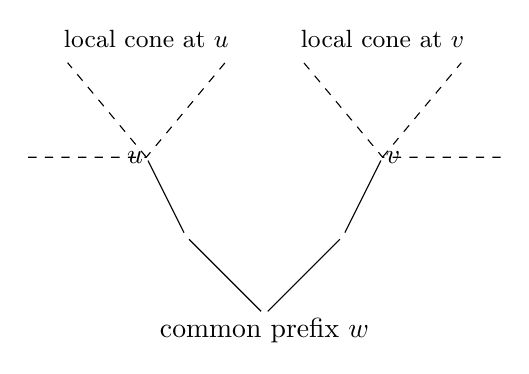
\begin{tikzpicture}[scale=1.0, every node/.style={inner sep=1pt}]
		% Common causal past
		\node (root) at (0,0) {};
		\node (a1)   at (-1,1) {};
		\node (b1)   at (1,1) {};

		% Two divergent prefixes u and v
		\node (u) at (-1.5,2) {};
		\node (v) at (1.5,2) {};

		% Subcones below u
		\draw[dashed] (-3,2) -- (-1.5,2) -- (-0.5,3.2);
		\draw[dashed] (-1.5,2) -- (-2.5,3.2);

		% Subcones below v
		\draw[dashed] (3,2) -- (1.5,2) -- (0.5,3.2);
		\draw[dashed] (1.5,2) -- (2.5,3.2);

		% Edges in prefix tree
		\draw (root) -- (a1);
		\draw (root) -- (b1);
		\draw (a1) -- (u);
		\draw (b1) -- (v);

		% Labels
		\node[left]  at (-1.5,2) {$u$};
		\node[right] at (1.5,2) {$v$};
		\node[below] at (0,0) {common prefix $w$};

		\node at (-1.5,3.5) {\small local cone at $u$};
		\node at (1.5,3.5) {\small local cone at $v$};
	\end{tikzpicture}
	\caption{Two Dyck prefixes $u$ and $v$ diverging from a shared ancestor $w$.
		Dashed regions indicate the local Catalan cones rooted at $u$ and $v$.
		Cones nest along causal chains and diverge after branching points, producing
	a family of local, relocatable causal geometries on the Catalan substrate.}
	\label{fig:multiple-cones}
\end{figure}

\subsection{Summary}
The Catalan substrate supports a discrete causal geometry determined entirely
by recursive constraint. Without introducing a manifold, metric, or causal
relation by fiat, it yields:
\begin{itemize}
	\item a partial order interpretable as causality,
	\item a cone-shaped causal envelope,
	\item intrinsic bounds on spatial extension,
	\item well-defined constant-time layers.
\end{itemize}
Subsequent sections place dynamical rules---quantum amplitudes and
computational reduction---on this geometry.

\section{Recursive Pairing and Universal Computation}
\label{sec:computation}

\subsection{Pairs expansion}

\paragraph{Catalan Structure as the Space of Program Possibilities.}

The Catalan family---Dyck paths, full binary trees, and balanced-parenthesis
expressions---forms the free magma on a single binary constructor. As observed
in foundational work on the $\lambda$-calculus and combinatory logic
\cite{CurryFeys1958,barendregt84}, every computable program has a canonical
representation as a finite binary application tree: internal nodes encode
application; leaves encode atomic symbols or combinators. Conversely, any finite
binary tree equipped with leaf labels denotes a unique program modulo surface
syntax. Thus the infinite Catalan tree is not merely a combinatorial object but
the structural possibility space of all programs expressible in any
Turing-complete functional calculus.

This observation also extends to operational semantics. Standard reductions
(such as $\beta$-reduction or SKI contraction) are local rewrite rules on binary
trees, and the pairs-expansions of combinators remain within the Catalan family.
Accordingly, a program, its intermediate expansion frames, and each permissible
reduction schedule are all representable as paths through a single Catalan
substrate. Selecting a program shape or selecting a specific reduction history
is therefore equivalent to selecting a path in the Catalan tree. In this sense
the Catalan substrate uniformly encodes program syntax, program semantics, and
the full ensemble of admissible computational histories.

\begin{proposition}[Catalan Universality for Program Structure]
	\label{prop:catalan-programs}
	Let $\mathcal{C}$ denote the Catalan family of finite full binary trees.
	Every program in any Turing-complete functional calculus (such as the
	$\lambda$-calculus or SKI) admits a canonical representation as an element of
	$\mathcal{C}$ with leaf labels drawn from a finite alphabet. Conversely,
	every labeled element of $\mathcal{C}$ denotes a unique program modulo surface
	syntax. Furthermore, standard operational semantics (including
	$\beta$-reduction and SKI contraction) act as local rewrite rules that
	preserve membership in $\mathcal{C}$. Thus a program, its syntactic
	expansions, and every admissible reduction history correspond to paths within
	the Catalan substrate.
\end{proposition}
\noindent
A proof sketch and illustrative examples are provided in
Appendix~\ref{appendix:computational-foundations}.

\paragraph{Two canonical parenthesis encodings.}
There are (at least) two particularly useful parenthesis-only encodings of a
full binary tree:

\begin{itemize}
  \item \textbf{Dyck encoding} (``walk'' view): balanced parentheses of length
    $2t$, naturally adapted to height profiles and scaling limits.
  \item \textbf{Pairs (S-expression) encoding} (``cons'' view): write each leaf
    as \texttt{()} and each internal node as a parenthesized pair of its two
    children, i.e.\ $T=(L,R)\mapsto (\texttt{enc}(L)\,\texttt{enc}(R))$.  This is
    a variable- and label-free Lisp-style representation with \texttt{()} as the
    only atom.
\end{itemize}

In particular, in the \emph{pairs} encoding, the smallest object is the empty
pair \texttt{()}, and the smallest nontrivial \emph{binary} object is
\texttt{(()())}, i.e.\ a root pair whose two children are leaves.  In the Dyck
encoding, the semilength-$1$ object is \texttt{()}, since Dyck words begin only
after the first matched pair exists.

\subsection{A small tier shown three ways (Dyck / tree / pairs)}
Figure~\ref{fig:trees-n3-tikz} augments the standard Dyck-$n=3$ list by
displaying, for the \emph{same} five Catalan shapes, the corresponding pairs
(S-expression) encodings.

\begin{figure}[H]
  \centering
  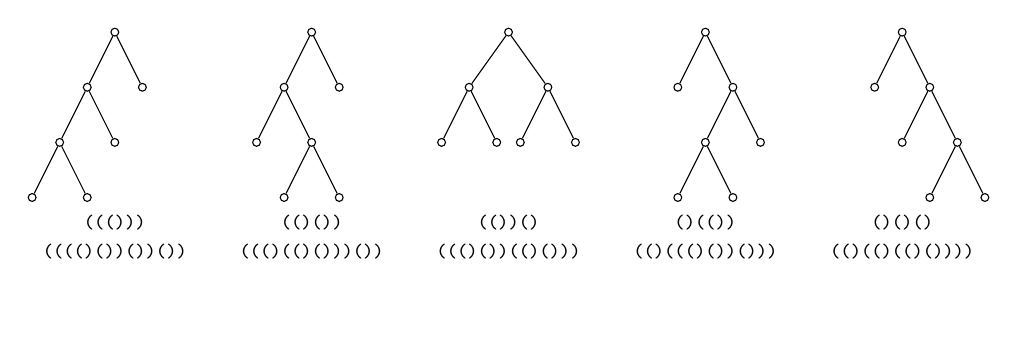
\begin{tikzpicture}[
    level 1/.style={level distance=7mm,sibling distance=7mm},
    level 2/.style={level distance=7mm,sibling distance=7mm},
    every node/.style={circle,draw,inner sep=1pt,minimum size=2pt}
    ]
    % Order: ((())), (()()), (())(), ()(()), ()()()
    % Pairs encodings (canonical): 
    % ((())) -> (((()())())())
    % (()()) -> ((()(()()))())
    % (())() -> ((()())(()()))
    % ()(()) -> (()((()())()))
    % ()()() -> (()(()(()())))
    %
    % 1) ((()))
    \begin{scope}[shift={(-5,0)}]
      \node {}
        child { node {}
          child { node {}
            child { node {} }
            child { node {} }
          }
          child { node {} }
        }
        child { node {} };
      \node[draw=none,align=center] at (0,-2.6)
      {\scriptsize\texttt{((()))}\\[-0.6mm]\scriptsize\texttt{(((()())())())}};
    \end{scope}
    % 2) (()())
    \begin{scope}[shift={(-2.5,0)}]
      \node {}
        child { node {}
          child { node {} }
          child { node {}
            child { node {} }
            child { node {} }
          }
        }
        child { node {} };
      \node[draw=none,align=center] at (0,-2.6)
      {\scriptsize\texttt{(()())}\\[-0.6mm]\scriptsize\texttt{((()(()()))())}};
    \end{scope}
    % 3) (())()
    \begin{scope}[
      shift={(0,0)},
      level 1/.style={level distance=7mm,sibling distance=10mm}
      ]
      \node {}
        child { node {}
          child { node {} }
          child { node {} }
        }
        child { node {}
          child { node {} }
          child { node {} }
        };
      \node[draw=none,align=center] at (0,-2.6)
      {\scriptsize\texttt{(())()}\\[-0.6mm]\scriptsize\texttt{((()())(()()))}};
    \end{scope}
    % 4) ()(())
    \begin{scope}[shift={(2.5,0)}]
      \node {}
        child { node {} }
        child { node {}
          child { node {}
            child { node {} }
            child { node {} }
          }
          child { node {} }
        };
      \node[draw=none,align=center] at (0,-2.6)
      {\scriptsize\texttt{()(())}\\[-0.6mm]\scriptsize\texttt{(()((()())()))}};
    \end{scope}
    % 5) ()()()
    \begin{scope}[shift={(5,0)}]
      \node {}
        child { node {} }
        child { node {}
          child { node {} }
          child { node {}
            child { node {} }
            child { node {} }
          }
        };
      \node[draw=none,align=center] at (0,-2.6)
      {\scriptsize\texttt{()()()}\\[-0.6mm]\scriptsize\texttt{(()(()(()())))}};    
    \end{scope}
  \end{tikzpicture}
  \vspace{-2.5em}
  \caption{The five Catalan shapes at tier $t=3$ shown as (i) Dyck words,
  (ii) full binary trees, and (iii) pairs (S-expression) encodings in which each
  leaf is \texttt{()} and each internal node is a parenthesized pair of its two
  children (as if one were looking "down into" the tree). These are three
  coordinate systems for the same underlying Catalan objects.}
  \label{fig:trees-n3-tikz}
\end{figure}

\subsection{Connection to \texorpdfstring{$\lambda$}{lambda}-calculus and SKI}

Binary trees are a standard representation of $\lambda$-terms and SKI
combinators \cite{church33,curry58,barendregt84}. Variables may be represented
by leaf positions, abstraction by structural capture, and application by tree
composition. Under the pairs expansion, each Dyck tree canonically determines an
unlabeled application graph. When variables are suppressed, the resulting graphs
coincide with the structure graphs used in combinatory logic. No additional
primitives beyond recursive pairing are required to obtain this representation.

Choosing a finite set of tree patterns to represent the SKI combinators and
interpreting local tree rewrites as SKI reduction therefore equips the Catalan
substrate with a standard universal calculus: every partial recursive function
can be encoded as an SKI term, and hence by a finite Dyck tree, and every
computation corresponds to a sequence of local tree transformations. In this
sense, the Catalan substrate is \emph{computationally universal}. What is new
here is that the same underlying objects simultaneously carry a causal and
geometric interpretation.

\subsection{Reduction and local collapse}

In the computational interpretation, reduction corresponds to local pattern
replacement. A redex occupies a finite region of a tree and may be reduced
without reference to distant subtrees. This locality mirrors the causal
structure established in Section~\ref{sec:catalan_cone}. From the perspective
of the Catalan lattice, reduction may be viewed as \emph{collapse}: a locally
ambiguous structure is replaced by a simpler one consistent with the global
constraint. Importantly, collapse does not alter causal ancestry; it refines an
already-admissible history. For standard calculi (e.g.\ $\lambda$/SKI),
confluence ensures uniqueness of normal forms when they exist, and more locally
reductions supported on disjoint subtrees commute. This computational fact will
later support an interpretation of spacelike commutativity.

\subsection{Summary}

Recursive pairing suffices to encode universal computation. Via the pairs
expansion, Dyck trees and application graphs are two views of the same
structure. Local computational reduction aligns naturally with causal locality
on the Catalan light cone.

\section{Quantum Amplitudes on the Catalan Lattice}
\label{sec:amplitudes}

\subsection{Histories as paths}

Interpreting Dyck paths as admissible histories motivates assigning weights to
each history.  Let $\mathcal{D}_t$ denote the set of Dyck paths of tier $t$. A
state at tier $t$ may be represented as a formal superposition of histories

\[
	\Psi_t = \sum_{w \in \mathcal{D}_t} \psi(w)\,|w\rangle .
\]

Local extensions of a Dyck path correspond to admissible future steps. Thus,
time evolution is governed by transitions that respect the Dyck constraint.

\subsection{Observables, projection, and coherent summation}

Fix a tier $t$ and consider the set $\mathcal D_t$ of Dyck paths of semilength
$t$. Each $w\in\mathcal D_t$ represents a complete admissible history at discrete
time $t$, with an associated height profile
\[
H_w : \{0,1,\dots,2t\} \to \mathbb Z_{\ge 0}.
\]
An observable is defined as a deterministic coarse-graining
\[
f : \mathcal D_t \to \mathcal X,
\]
where $\mathcal X$ is a discrete set of outcomes corresponding to a chosen
equivalence relation on histories. An outcome $x\in\mathcal X$ corresponds to
the equivalence class $f^{-1}(x)\subset\mathcal D_t$ of histories.  By
construction, such a projection discards information: many distinct histories
may be identified as the same observable outcome.

With no additional structure imposed, the natural measure on $\mathcal D_t$ is
uniform counting. The induced distribution on the outcome space $\mathcal X$ is
therefore the pushforward of the uniform counting measure,
\[
N(x) := \#\{w\in\mathcal D_t : f(w)=x\}.
\]
Even with uniform weight on histories, the induced distribution on $\mathcal X$
is generically non-uniform, reflecting the combinatorial geometry of the
projection rather than any imposed dynamics.

A discrete analogue of an integral along a history is given by the step-sum of
the height profile,
\[
A(w) := \sum_{k=0}^{2t-1} H_w(k),
\]
which measures the cumulative dwell time at nonzero height. This quantity
depends on the full distribution of height along the path, not merely on
extrema such as maximum height or peak count.

From this additive structural functional one may define a complex phase
\[
\theta(w) := \alpha\,A(w),
\qquad
\psi(w) := e^{i\theta(w)},
\]
where $\alpha$ is a global scale parameter. No per-path phase assignment is
introduced; distinct phases arise solely from differences in the distribution of
height over the history.

Given an observable $f$, the complex amplitude associated with an outcome
$x\in\mathcal X$ is the coherent sum
\[
\Psi(x) := \sum_{w:\,f(w)=x} \psi(w),
\]
and observed probabilities are obtained by normalization of squared magnitudes,
\[
P(x) = \frac{|\Psi(x)|^2}{\sum_{x'\in\mathcal X}|\Psi(x')|^2}.
\]
Thus histories that are indistinguishable under the observable $f$ are combined
prior to squaring, while distinguishable histories are not. Interference is
therefore a generic consequence of assigning complex weights to histories and
summing coherently over coarse-grained equivalence classes before applying the
Born rule.

\paragraph{Optional: coarse-graining entropy.}
Appendix~\ref{appendix:technical-notes} records an optional entropy bookkeeping
for coarse-grainings and collapse counts.

\subsection{Path integrals and conditioned walks}

Dyck paths are random walks conditioned to remain nonnegative and return to
zero. Classical results show that, when rescaled appropriately, ensembles of
such paths converge to Brownian excursions \cite{le-gall05,janson07}.
Assigning equal weight to all admissible paths yields a discrete path integral.
More general amplitude assignments may depend on local features such as height
or curvature, provided the Dyck constraint is preserved.

\begin{figure}[h]
	\centering
	\begin{tikzpicture}[scale=0.7]
		% axes
		\draw[->] (0,0) -- (13,0) node[below] {$k$};
		\draw[->] (0,0) -- (0,6) node[left] {$H_k$};
		% sample Dyck path (semilength 6)
		\draw[thick]
			(0,0) -- (1,1) -- (2,2) -- (3,3) -- (4,2) -- (5,3) -- (6,4)
			-- (7,3) -- (8,2) -- (9,3) -- (10,2) -- (11,1) -- (12,0);
		% labels
		\node[below] at (0,0) {0};
		\node[below] at (12,0) {$2n$};
		\node[above right] at (3,3) {\small Dyck walk};
		% schematic smooth excursion overlay
		\draw[dashed] plot[smooth] coordinates {
				(0,0) (2,1) (4,2.8) (6,4.2) (8,2.5) (10,1.2) (12,0)
			};
		\node[right] at (12,4.2) {\small Brownian excursion (scaling limit)};
	\end{tikzpicture}
	\caption{A Dyck path as a nearest-neighbour walk $(H_k)$ constrained to stay
		nonnegative and return to zero at time $2n$.
		Under diffusive rescaling of $k$ and $H_k$, ensembles of such paths converge
		to Brownian excursions, providing the bridge to the heat and Schr\"odinger
	equations discussed in the text.}
	\label{fig:dyck-walk-excursion}
\end{figure}

\paragraph{Optional stratifications.}
Appendix~\ref{appendix:technical-notes} discusses Narayana stratification by
peak count as an optional organizing tool.

\subsection{Discrete path-integral formulation}

The preceding constructions admit a direct interpretation as a discrete path
integral on the Catalan light cone. Fix a tier $t$ and an observable
$f:\mathcal D_t\to\mathcal X$, where $\mathcal X$ is a finite set of outcomes
corresponding to a chosen coarse-graining of histories. Each Dyck path
$w\in\mathcal D_t$ represents a complete admissible history, and the projection
$f$ determines which distinctions between histories are retained and which are
discarded.

Define a complex weight for each history by
\[
\psi(w) = e^{i\alpha A(w)},
\]
where
\[
A(w) = \sum_{k=0}^{2t-1} H_w(k)
\]
is the discrete height integral introduced above. The amplitude associated with
an observable outcome $x\in\mathcal X$ is then
\[
\Psi(x) = \sum_{w:\,f(w)=x} e^{i\alpha A(w)}.
\]


This expression is formally identical to a path integral: the amplitude is a sum
over all admissible histories compatible with the observable outcome, with each
history contributing a phase determined by an additive functional. No continuum
limit, action functional, or variational principle is assumed at this stage; the
structure arises purely from discrete combinatorics.

Several features commonly associated with continuum path integrals are already
present:

\begin{enumerate}[label=(\roman*)]
\item \textbf{Sum over histories.}
All admissible Dyck paths consistent with the observable contribute. The Dyck
constraint enforces causal admissibility in the same way that restrictions on
allowed paths do in relativistic path integrals.

\item \textbf{Additive phase functional.}

The quantity $A(w)$ is additive under concatenation of path segments and depends
only on the local height increments. It therefore plays the role of a discrete
action accumulated along the history.

\item \textbf{Interference from coarse-graining.}
Interference arises precisely because the observable $f$ fails to distinguish
between certain histories. Histories that are identified by the projection are
summed coherently, while those distinguished by the observable are not.

\item \textbf{Gauge redundancy.}
Different Dyck paths may correspond to the same abstract computation or the same
coarse-grained structure, differing only by the ordering of spacelike-separated
updates. The path integral sums coherently over such gauge-equivalent histories,
while observable probabilities depend only on the resulting amplitudes.
\end{enumerate}

From this perspective, the Catalan lattice provides a discrete realization of
the sum-over-histories principle in which both the space of histories and the
phase functional are combinatorially well defined. In the next subsection we
show that, under appropriate scaling limits, this discrete formulation
converges to familiar continuum descriptions governed by diffusion and
Schr\"odinger dynamics.

Concrete physical measurements may be modeled by choosing observables that
retain geometric features of a history (such as transverse displacement at a
fixed tier). No such spatial interpretation, however, is required for the
formal development.

For readers seeking a concrete intuition for how this discrete
sum-over-histories mechanism produces interference,
Appendix~\ref{appendix:doubleslit} sketches a finite thought experiment
analogous to the double-slit experiment.

\subsection{Scaling of the area phase in the continuum limit}
\label{subsec:phase-scaling}

The interference mechanism above assigns each history $w\in\mathcal D_n$ a
complex weight $\psi(w)=e^{i\alpha A(w)}$ with discrete area functional
\[
A(w) := \sum_{k=0}^{2n-1} H_w(k),
\]
where $H_w(k)$ is the height after $k$ steps.

To relate this discrete phase to the diffusion scaling limit, introduce the
rescaled height process on $[0,1]$,
\[
X^{(n)}(\tau) := n^{-1/2} H_w(\lfloor 2n\tau\rfloor), \qquad 0\le \tau \le 1.
\]
Under the standard Dyck-to-Brownian-excursion scaling, $X^{(n)} \Rightarrow X$
in distribution, where $X$ is a Brownian excursion on $[0,1]$.

The discrete area rescales as a Riemann sum:
\[
\frac{1}{2n^{3/2}}A(w)
= \frac{1}{2n}\sum_{k=0}^{2n-1} n^{-1/2}H_w(k)
\;\Longrightarrow\;
\int_0^1 X(\tau)\,d\tau.
\]
Consequently, a nontrivial continuum phase is obtained by scaling $\alpha$ with
$n$ as
\[
\alpha_n := \frac{\lambda}{2n^{3/2}},
\]
so that
\[
e^{i\alpha_n A(w)}
\;\Longrightarrow\;
\exp\!\Big(i\lambda\int_0^1 X(\tau)\,d\tau\Big).
\]

This makes explicit that the discrete coherent sum with additive functional
$A(w)$ converges to a continuum functional weight. In particular, when one
passes from uniform counting of conditioned walks to diffusion limits, inserting
the exponential of a time-integrated functional corresponds (at the PDE level)
to adding a potential term (via the standard Feynman--Kac mechanism). Setting
$\lambda=0$ recovers the unweighted scaling limit discussed in the next
subsection.

\subsection{Diffusion limit}
\label{sec:continuum-limit}

Let $n\to\infty$ and rescale time and height by

\[
	t \mapsto n\tau, \qquad h \mapsto \sqrt{n}\,x .
\]

Under this scaling, the probability density $\rho(\tau,x)$ for conditioned walks
converges in law to that of a Brownian excursion on $x\ge0$. At the PDE level,
the associated continuum evolution is governed by the heat operator on the
half-line, with the Dyck conditioning encoded by appropriate
boundary/conditioning at $x=0$. In particular, one obtains a heat equation of
the form

\begin{equation}
	\partial_\tau \rho = \frac{1}{2}\,\partial_x^2 \rho,
\end{equation}

with the boundary/conditioning determined by the chosen scaling limit and
conditioning. Full derivations may be found in \cite{le-gall05,janson07}.

\subsection{Schr\"odinger equation}

More formally, if $\rho(\tau,x)$ denotes the real heat kernel on $x\ge 0$,
analytic continuation in the diffusion parameter, $\tau \mapsto it$, produces a
complex-valued kernel $\psi(t,x)$ satisfying the free Schr\"odinger equation

\begin{equation}
	i\partial_t \psi = -\frac{1}{2}\,\partial_x^2 \psi.
\end{equation}

Boundary conditions at $x=0$ are carried over from the diffusive regime (e.g.\
reflecting or absorbing), and the choice of boundary does not affect the
existence of the continuum limit itself. Thus, quantum wave dynamics arises here
as the analytic continuation of diffusive propagation on the Catalan lattice, in
line with the classical connection between diffusion and Schr\"odinger evolution
\cite{feynman-hibbs65,kac49}. No separate quantization procedure is required;
the wave equation is inherited from the scaling limit of constrained
combinatorial growth.

\section{Locality, Commutation, and Interaction}
\label{sec:locality}

\subsection{Disjoint subtrees}

Two subtrees of a Dyck tree that share no common ancestor beyond a given prefix
are causally independent. Operations localized to one subtree do not affect the
other. In the computational interpretation, this corresponds to independent
reductions. In the amplitude interpretation, it corresponds to commuting
operators acting on spacelike-separated regions. Multiple Dyck paths may
represent the same abstract computation or the same coarse-grained geometry.
Such redundancies may be quotiented out without changing observable
predictions, yielding equivalence classes of histories. This redundancy plays a
role analogous to gauge symmetry: distinct internal descriptions correspond to
the same external behavior.

Operationally, gauge here means a redundancy in the description of histories.
For a fixed initial tree, consider the class of causal histories that apply the
same multiset of local reductions but differ only in the temporal ordering of
reductions supported on disjoint subtrees. Such histories are gauge-equivalent:
they represent the same physical pattern of events, and their linear orderings
are related by commuting spacelike-separated updates. The resulting equivalence
classes (gauge orbits) play the role of physical histories, while genuinely
different choices of which reductions to actualize belong to distinct orbits and
define the nontrivial branching structure of the multiway reduction graph.

\begin{figure}[h]
  \centering
  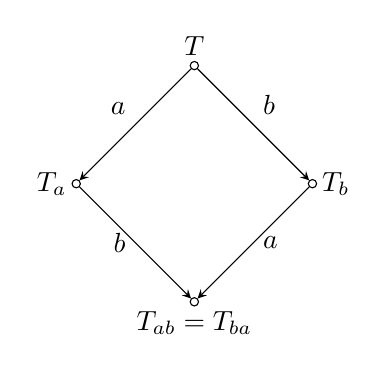
\begin{tikzpicture}[>=stealth]
    % nodes
    \node[circle,draw,inner sep=1pt,minimum size=3pt] (T)   at (0,0)    {};
    \node[circle,draw,inner sep=1pt,minimum size=3pt] (Ta)  at (-1.5,-1.5) {};
    \node[circle,draw,inner sep=1pt,minimum size=3pt] (Tb)  at (1.5,-1.5)  {};
    \node[circle,draw,inner sep=1pt,minimum size=3pt] (Tab) at (0,-3)   {};

    % labels
    \node[above] at (T)   {$T$};
    \node[left]  at (Ta)  {$T_a$};
    \node[right] at (Tb)  {$T_b$};
    \node[below] at (Tab) {$T_{ab}=T_{ba}$};

    % arrows
    \draw[->] (T)  -- node[above left]  {$a$} (Ta);
    \draw[->] (T)  -- node[above right] {$b$} (Tb);
    \draw[->] (Ta) -- node[left]        {$b$} (Tab);
    \draw[->] (Tb) -- node[right]       {$a$} (Tab);
  \end{tikzpicture}
  \caption{Local diamond for commuting disjoint updates. Starting from a
  common state $T$, two spacelike-separated reductions $a$ and $b$ can be
  applied in either order, yielding intermediate states $T_a$ and $T_b$
  but the same final state $T_{ab}=T_{ba}$. The two intermediate events
  are spacelike-separated: they share a common past ($T$) and a common
  future ($T_{ab}$) but no causal edge between them. This expresses
  microcausality on the Catalan substrate: local updates supported on
  disjoint subtrees commute and differ only by a gauge choice of temporal
  ordering.}
  \label{fig:disjoint-subtrees}
\end{figure}

(See Appendix~\ref{appendix:computational-foundations}, and in particular
Lemma~\ref{lem:causal-consistency}, for a formal statement and proof sketch
of the corresponding disjoint-commutation property.)

\subsection{Collapse and selection}
Both computation and amplitude propagation require selection:
\begin{itemize}
	\item computational reduction chooses a redex,
	\item measurement-like selection chooses an observable outcome, corresponding
		to an equivalence class under the chosen projection.
\end{itemize}
In the Catalan substrate, selection operates locally, refining rather than
destroying structure. The global constraint ensures consistency after
selection. The formal development of collapse probabilities lies beyond the
scope of this paper and is treated here only structurally.

\subsection{Summary}
Locality, commutation, and interaction emerge directly from the causal and
recursive structure of the Catalan lattice. The same principles underlie both
computational reduction and quantum amplitude propagation.

\section{Discussion and Limitations}
\label{sec:discussion}

The results presented here establish a shared structural basis for causal
geometry, quantum dynamics, and computation. Several limitations should be
emphasized:
\begin{itemize}
	\item Physical constants and interactions are not derived.
	\item Only free (noninteracting) wave dynamics appears explicitly.
	\item Collapse probabilities are not fixed uniquely by the structure.
\end{itemize}
These limitations reflect a deliberate restriction of scope. The goal has been
to isolate the minimal recursive structure common to multiple domains, not to
provide a complete physical theory.

\subsection{Relation to discrete quantum gravity}

Similar scaling behavior appears in two-dimensional quantum gravity and random
surface models. In particular, Causal Dynamical Triangulations (CDT) enforce a
preferred foliation and causal constraint that parallels the prefix order of
Dyck paths \cite{ambjorn01,ambjorn12}. In CDT, the continuum limit is taken
after summing over causally admissible triangulations. Here the admissible
structures are Dyck paths rather than triangulations, but the organizing
principle---the restriction to histories that respect a causal growth rule---is
closely analogous.

\section{Conclusion}
\label{sec:conclusion}

This paper has examined the Catalan family of recursive structures as a common
substrate for causal geometry, quantum amplitude propagation, and computation.
The Dyck constraint induces a natural causal order and a discrete cone-shaped
geometry exhibiting light-cone--like bounds. Classical invariance principles
show that ensembles of admissible histories converge in the continuum limit to
Brownian excursions, leading to diffusive continuum limits governed by the heat
operator (with the Dyck conditioning encoded on the half-line) and, under
analytic continuation, the free Schr\"odinger equation. Through the pairs expansion, the
same structures encode universal computation via $\lambda$-calculus and SKI
combinators. These correspondences require no additional primitives beyond
recursive pairing and constraint.
Spacetime-like geometry, wave dynamics, and computation emerge as complementary
aspects of a single recursive system. Several open problems remain, including
the incorporation of interaction terms, the determination of collapse
probabilities, and the connection to physical constants. The results presented
here establish a minimal and structurally unified foundation upon which such
extensions may be explored.

\appendix

\section{Coordinate Charts and Continuum Comparisons}
\label{appendix:coordinate-charts}

This appendix collects optional coordinate embeddings and continuum comparisons
used for intuition; the combinatorial results in the main text do not depend on
these constructions.

\subsection{Coordinate charts on the Catalan cone}
\label{sec:coordinate-charts}

\begin{remark}[Notation hygiene]
\label{rem:notation-hygiene}
To avoid collisions, the \emph{tier} (semilength) of a completed history is
denoted by $n$. A \emph{prefix length} is denoted by $k\in\{0,1,\dots,2n\}$.
Within this subsection only, the symbols $(t_k,x_k)$ denote an \emph{embedded}
spacetime chart derived from cumulative counts (Definition~\ref{def:null-counts}),
and should not be confused with the tier index $n$ used elsewhere.
\end{remark}

\paragraph{The Catalan cone as the master object.}
Let $\mathcal{C}$ denote the set of Dyck prefixes (balanced-parentheses
\emph{prefixes} that never go below height $0$), partially ordered by extension:
$p\preceq q$ iff $q$ has prefix $p$. A completed history is a maximal element
$w\in\mathcal{D}_n\subset\mathcal{C}$ of semilength $n$.
For any prefix $p\in\mathcal{C}$, the future
\[
\mathcal{C}(p)\;:=\;\{\,q\in\mathcal{C}: p\preceq q\,\}
\]
is canonically a ``local cone'' rooted at $p$: the same growth law, re-centered.
Thus there is a single substrate $\mathcal{C}$ (and its re-rootings), and
different ``cones'' arise from different coordinate charts or coarse-grainings
of this same object.

\paragraph{Two cumulative counts and a light-cone chart.}
The most rigid chart on $\mathcal{C}$ is obtained by tracking the cumulative
numbers of opens and closes.

\begin{definition}[Null counts and embedded coordinates]
\label{def:null-counts}
Fix a Dyck word $w\in\mathcal{D}_n$, and let $w[1\!:\!k]$ denote its length-$k$
prefix. Define
\[
u(k)\;:=\;\#\{\texttt{(}\text{ in }w[1\!:\!k]\},\qquad
v(k)\;:=\;\#\{\texttt{)}\text{ in }w[1\!:\!k]\}.
\]
The Dyck admissibility constraint is $u(k)\ge v(k)$ for all $k$, and completion
is $u(2n)=v(2n)=n$. Define the height (frontier) process
\[
H(k)\;:=\;u(k)-v(k)\;\ge\;0,
\]
and the embedded ``spacetime'' coordinates
\[
t_k\;:=\;\frac{u(k)+v(k)}{2}\;=\;\frac{k}{2},\qquad
x_k\;:=\;\frac{u(k)-v(k)}{2}\;=\;\frac{H(k)}{2}.
\]
Equivalently $u=t_k+x_k$ and $v=t_k-x_k$ (a discrete null-coordinate form).
\end{definition}

Under this embedding, each symbol advances time and changes space by one unit
(up to the $1/2$ normalization):
\[
\texttt{(}:\ (t,x)\mapsto (t+\tfrac12,\ x+\tfrac12),\qquad
\texttt{)}:\ (t,x)\mapsto (t+\tfrac12,\ x-\tfrac12).
\]
Hence the path stays inside the cone $|x_k|\le t_k$, with the boundary $x_k=0$
representing zero frontier (no outstanding opens).

\paragraph{Why ``return to $0$'' is not ``return to the origin.''}
The completion constraint $H(2n)=0$ means only that the \emph{imbalance} vanishes:
every open has been matched by a close. In spacetime coordinates, the endpoint is
\[
(t_{2n},x_{2n})\;=\;\bigl(n,0\bigr),
\]
not $(0,0)$. Thus a history expands monotonically in $t$ (prefix length grows),
while the spatial coordinate $x$ is a \emph{frontier variable} that eventually
returns to $0$ because no unfinished structure may remain at completion.

\paragraph{Pairs, trees, and $S$-expressions are identical structure.}
A Dyck word $w$ can be read as a parenthesized $S$-expression skeleton, and it
already \emph{is} a rooted ordered tree:
matched parenthesis pairs are nodes; containment defines parent/child; and
left-to-right order in the string gives sibling order.
For example, $w=\texttt{(()())}$ has one outer pair (the root) containing two
inner pairs (two leaves). Under this identification, the height $H(k)$ is the
number of currently-open pairs---the size of the \emph{active frontier} of the
tree under construction.

\paragraph{Evaluation ``return'' as frontier discharge.}
If evaluation is recorded at the level of control (continuations), then entering
a subproblem pushes a context frame and finishing it pops that frame. In a
well-bracketed evaluation regime, this push/pop trace is Dyck, and the same
counts $(u(k),v(k))$ track control events. The embedded coordinate $x_k$
therefore measures continuation depth (pending contexts), and the return to
$x=0$ at termination is the emptying of the continuation stack: no pending
contexts remain. Value return is mediated by this control return; the Dyck
``return'' is fundamentally the discharge of outstanding obligations.

\paragraph{Breadth as a different projection (history-level, not frontier-level).}
Statistics such as breadth $r(w)$ summarize a \emph{completed} history by the
maximum size of a constant-depth slice in its associated tree. This is a
coarse-graining of $w$ (many distinct histories share the same $(n,r)$), and it
should be distinguished from the frontier coordinate $x_k$, which is an
instantaneous depth/obligation variable along a single prefix trajectory.

\paragraph{Summary of the two readings.}
There is one substrate $\mathcal{C}$ (and its re-rooted futures $\mathcal{C}(p)$).
Two useful ``cone'' pictures arise from:
(i) the embedded prefix trajectory $(t_k,x_k)$ derived from null counts
(pathwise frontier dynamics), and
(ii) history-level projections such as $(n,r(w))$ (coarse geometric envelope).
The pairs/tree/$S$-expression view does not introduce a new object; it is an
identity of representations of the same Catalan structure.

\subsection{Dyck Coordinates, Lorentz Geometry, and Computational Proper Time}
\label{subsec:dyck-lorentz-computation}

\begin{remark}[Indices and coordinate conventions]
Throughout, $n$ denotes the tier (semilength) of a completed Dyck history.
Within this subsection, $k\in\{0,1,\dots,2n\}$ denotes a \emph{step index} along a
single history, and $m$ denotes the number of \emph{collapse events} (local redex
contractions) performed by a chosen evaluation strategy.
\end{remark}

A Dyck history $w\in\mathcal D_n$ induces an integer-valued nearest-neighbour
walk $(H_k)_{k=0}^{2n}$ (the height / nesting depth signal) with
\[
H_{k+1}=H_k\pm 1,\qquad H_0=0,\qquad H_k\ge 0,\qquad H_{2n}=0.
\]
Define the rescaled coordinates
\[
t_k:=\frac{k}{2},\qquad x_k:=\frac{H_k}{2},
\]
so that each parenthesis advances time by $\tfrac12$ and changes the transverse
coordinate by $\pm\tfrac12$:
\[
\texttt{(}:\ (t,x)\mapsto (t+\tfrac12,\ x+\tfrac12),\qquad
\texttt{)}:\ (t,x)\mapsto (t+\tfrac12,\ x-\tfrac12).
\]
For any walk with steps $(\Delta t,\Delta x)=(\tfrac12,\pm\tfrac12)$ one has the
kinematic cone bound $|x_k-x_0|\le t_k-t_0$. In the Dyck case, the additional
constraint is one-sided: $x_k\ge 0$ for all $k$, together with the endpoint
condition $x_{2n}=0$. Thus Dyck histories occupy the right half of a discrete
light cone and return to the axis only at completion.

Introduce discrete null coordinates (compare Definition~\ref{def:null-counts})
\[
u:=t+x,\qquad v:=t-x.
\]
In continuum $(1+1)$-dimensional Minkowski space, a Lorentz boost with rapidity
$\eta$ acts linearly as
\begin{equation}
u' = e^{\eta} u,\qquad v' = e^{-\eta} v,
\label{eq:lightcone-boost}
\end{equation}
and transforming back to $(t,x)$ yields the standard Lorentz transformation
\begin{equation}
t' = \gamma (t - v_{\!L} x),\qquad x' = \gamma (x - v_{\!L} t),
\label{eq:lorentz-tx}
\end{equation}
where
\[
\gamma=\frac{1}{\sqrt{1-v_{\!L}^2}},\qquad v_{\!L}=\tanh\eta,
\]
in units $c=1$. The Minkowski interval
\begin{equation}
\mathrm{d}s^{2}=\mathrm{d}t^{2}-\mathrm{d}x^{2}
\label{eq:minkowski}
\end{equation}
is invariant under~\eqref{eq:lorentz-tx}. In this sense the step rule supplies a
discrete null-step kinematics, while the Dyck constraint supplies the boundary
and return conditions selecting the Catalan ensemble. We emphasize that generic
nontrivial boosts do not preserve the discrete Dyck lattice itself (the counts
$u,v$ are integers), so the Lorentz discussion here is a continuum comparison
for the embedded coordinates rather than a discrete symmetry claim.

\paragraph{Computational proper time.}
A reduction history carries an intrinsic progress parameter given by the count
of collapse events. Let $m$ be the number of local redex contractions performed
by an evaluation strategy up to a given stage, and define the \emph{computational
proper time}
\begin{equation}
\tau := \alpha\, m,
\label{eq:tau-discrete}
\end{equation}
where $\alpha>0$ is the characteristic scale associated with a single collapse.
In continuum Minkowski space, a parametrized world-line $(t(s),x(s))$ admits a
proper-time functional
\begin{equation}
\left(\frac{\mathrm{d}\tau}{\mathrm{d}s}\right)^{2}
=
\left(\frac{\mathrm{d}t}{\mathrm{d}s}\right)^{2}
-
\left(\frac{\mathrm{d}x}{\mathrm{d}s}\right)^{2},
\label{eq:proper-time-continuum}
\end{equation}
which is Lorentz-invariant under~\eqref{eq:lorentz-tx}. In the present discrete
setting, Equation~\eqref{eq:tau-discrete} is simply a well-defined event-count
parameter; the analogy is that collapse count plays the role of a proper-time
progress variable along a chosen computational history.

\section{Additional Technical Notes}
\label{appendix:technical-notes}

\subsection{Entropy of coarse-graining and information rate}

Fix a tier $t$ and an observable (deterministic coarse-graining)
$f:\mathcal D_t\to\mathcal X$. For $x\in\mathcal X$ write
\[
N(x)\;:=\;\#\{w\in \mathcal D_t: f(w)=x\},
\]
so that $f^{-1}(x)$ is the equivalence class of histories identified as the
same outcome.

\paragraph{Multiplicity entropy.}
Define the (microcanonical) entropy of the full ensemble at tier $t$ by
\[
S_t \;:=\; \log \#(\mathcal D_t),
\]
and the conditional entropy of an outcome $x$ by
\[
S(x) \;:=\; \log N(x).
\]
The information eliminated by selecting outcome $x$ is the entropy drop
\[
\Delta S(x)\;:=\; S_t - S(x)
\;=\; \log\!\Big(\frac{\#(\mathcal D_t)}{N(x)}\Big).
\]
(Any logarithm base may be used; base $2$ yields units of bits.)

\paragraph{Information rate as rate of possibility reduction.}
Let $k$ denote the number of selection events (local contractions) along a
history, and let computational proper time be $\tau=\tau_0 k$ for a fixed scale
$\tau_0>0$. We define the information rate associated with outcome $x$ to be the
information loss per unit computational proper time,
\[
R(x)\;:=\;\frac{\Delta S(x)}{\tau}.
\]
In the simplest case of a single event ($k=1$), this reduces to
$R(x)=\Delta S(x)/\tau_0$.

\begin{proposition}[Basic properties]
\label{prop:information-rate-basic}
For any observable $f:\mathcal D_t\to\mathcal X$:
\begin{enumerate}[label=(\roman*)]
\item (Nonnegativity) $\Delta S(x)\ge 0$ for all attainable $x\in\mathcal X$,
with equality iff $N(x)=\#(\mathcal D_t)$ (i.e.\ $f$ is constant on
$\mathcal D_t$).
\item (Additivity under independent factorization) If $\mathcal D_t$ factorizes
as a Cartesian product $\mathcal D_t \cong \mathcal D_t^{(1)}\times
\mathcal D_t^{(2)}$ and $f(w_1,w_2)=(f_1(w_1),f_2(w_2))$, then
\[
\Delta S(x_1,x_2)=\Delta S_1(x_1)+\Delta S_2(x_2).
\]
\end{enumerate}
\end{proposition}

\begin{proof}
(i) Since $1\le N(x)\le \#(\mathcal D_t)$ whenever $x$ is attainable, the ratio
$\#(\mathcal D_t)/N(x)\ge 1$, hence $\Delta S(x)\ge 0$, with equality exactly
when $N(x)=\#(\mathcal D_t)$.
(ii) Under the stated factorization, $N(x_1,x_2)=N_1(x_1)N_2(x_2)$ and
$\#(\mathcal D_t)=\#(\mathcal D_t^{(1)})\#(\mathcal D_t^{(2)})$, so $\Delta S$
splits as a sum.
\end{proof}

\paragraph{Gauge-invariant counting.}
When histories admit a redundancy under commuting spacelike-separated updates,
one may quotient $\mathcal D_t$ by the induced gauge equivalence relation
$\sim_g$ and define $\bar{\mathcal D}_t:=\mathcal D_t/\!\sim_g$. If $f$ is
gauge-invariant (constant on $\sim_g$-orbits), define
\[
\bar N(x):=\#\{[w]\in \bar{\mathcal D}_t : f(w)=x\},
\qquad
\bar{\Delta S}(x):=\log\!\Big(\frac{\#(\bar{\mathcal D}_t)}{\bar N(x)}\Big),
\]
and use $\bar{\Delta S}$ in place of $\Delta S$. This removes overcounting due
solely to reordering of independent collapses.

\subsection{Narayana stratification and structural modes}

Dyck paths admit a natural finite stratification by peak count. For
$w\in\mathcal D_t$, define its \emph{peak count} $K(w)$ as the number of indices
$k\in\{1,\dots,2t-1\}$ at which the Dyck word has an up-step immediately
followed by a down-step (equivalently, the number of local maxima of the height
profile $H_w(k)$). The Narayana numbers $N(t,k)$ count the number of Dyck paths
with $K(w)=k$, yielding the partition
\[
\mathcal D_t = \bigsqcup_{k=1}^{t} \mathcal D_{t,k},
\qquad
\mathcal D_{t,k} := \{w\in\mathcal D_t : K(w)=k\}.
\]

To make the notion of ``mode'' precise, embed each history into a finite
inner-product space. Let
\[
V_t := \mathbb R^{2t+1}, \qquad
H(w) := (H_w(0),\dots,H_w(2t)) \in V_t,
\]
with standard inner product
\[
\langle a,b\rangle := \sum_{j=0}^{2t} a_j b_j.
\]
Fix an orthonormal basis $\{\phi_m\}_{m=0}^{2t}$ of $V_t$ (for example, the
discrete cosine basis or the eigenvectors of the discrete Laplacian on the path
graph). The coefficients
\[
c_m(w) := \langle H(w), \phi_m\rangle
\]
define a spectral decomposition of the history $w$, with power spectrum
$P_m(w):=|c_m(w)|^2$.

The peak count $K(w)$ does not label a single spectral mode. Rather, it provides
a coarse combinatorial proxy for oscillatory complexity of the height signal. A
natural summary statistic for how a Narayana class distributes spectral weight
is the conditional mean spectrum
\[
\overline{P}_m(t,k) := \mathbb E\!\left[\,P_m(w)\mid w\in\mathcal D_{t,k}\right].
\]
Intuitively, larger $k$ tends to shift weight toward higher spectral indices
$m$, reflecting more frequent alternation of slopes; this heuristic may be used
as a discrete analogue of increased high-frequency content.

Finally, since the phase functional used in Section~\ref{sec:amplitudes} depends
on the full height profile (e.g.\ $\theta(w)=\alpha A(w)$), differences in peak
placement within a fixed Narayana class generally change $A(w)$ and hence the
phases appearing in coherent summation. Interference therefore depends both on
coarse stratification by $K(w)$ and on finer structural variation within each
class.

\section{A Double-Slit Thought Experiment on the Catalan Light Cone}
\label{appendix:doubleslit}

This appendix provides an illustrative thought experiment showing how the
discrete path-integral formalism developed in Section~\ref{sec:amplitudes}
exhibits interference in a setting analogous to the double-slit experiment.
The construction is entirely combinatorial and finite. No new assumptions,
dynamical rules, or continuum limits are introduced; the purpose is solely to
instantiate the formalism in a familiar narrative.

\subsection{Two sources as boundary-conditioned cones}

Consider two distinct Dyck prefixes $u_L$ and $u_R$ of equal length and height.
Each prefix induces a local Catalan cone of admissible continuations, as
described in Section~\ref{sec:multiplecones}. We refer to these as the left and
right source cones, although no spatial interpretation is assumed at this
stage.

Both cones are evolved to a common tier $n$, producing two ensembles of Dyck
paths of semilength $n$ that differ only in their initial boundary condition.
The admissible histories from both cones are evaluated relative to the same
observable defined below.

\subsection{Observable and indistinguishability}

Fix a tier $n$ and define an observable
\[
f : \mathcal D_n \to \mathcal X,
\]
where $\mathcal X$ is a discrete outcome space. The observable $f$ retains a
coarse-grained feature of each history (for example, a bin determined by the
mean height or total area) and discards all other information, including which
source cone the history originated from.

Interference arises precisely because histories originating from distinct cones
may be rendered indistinguishable by the observable. If the observable were to
retain source information, no interference would occur.

\subsection{Enumeration of histories at $n=3$}

At semilength $n=3$, the set $\mathcal D_3$ consists of the five Dyck words
\[
((())),\quad (()()),\quad (())(),\quad ()(()),\quad ()()().
\]

Each word $w$ determines a height profile $H_w(k)$ for $k=0,\dots,6$, and an
associated discrete area
\[
A(w) = \sum_{k=0}^{5} H_w(k).
\]

These quantities are listed in Table~\ref{tab:n3-dyck}.

\begin{table}[h]
\centering
\begin{tabular}{c c c}
Dyck word $w$ & height profile $H_w(k)$ & $A(w)$ \\ \hline
$((()))$   & $(0,1,2,3,2,1,0)$ & $9$ \\
$(()())$   & $(0,1,2,1,2,1,0)$ & $7$ \\
$(())()$   & $(0,1,2,1,0,1,0)$ & $5$ \\
$()(())$   & $(0,1,0,1,2,1,0)$ & $5$ \\
$()()()$   & $(0,1,0,1,0,1,0)$ & $3$
\end{tabular}
\caption{Dyck words at semilength $n=3$, with height profiles and discrete areas.}
\label{tab:n3-dyck}
\end{table}

\subsection{Coherent summation and interference}

Assign to each history the complex weight
\[
\psi(w) = e^{i\alpha A(w)},
\]
as in Section~\ref{sec:amplitudes}. Let $x\in\mathcal X$ be a fixed observable
outcome such that multiple histories from both source cones satisfy $f(w)=x$.

The amplitude associated with $x$ is
\[
\Psi(x) = \sum_{w:\,f(w)=x} e^{i\alpha A(w)}.
\]

Because the observable discards source information, contributions from the left
and right cones are summed coherently. Histories with equal area contribute the
same phase, while histories with different distributions of height contribute
distinct phases. Depending on the relative values of $A(w)$, the sum may exhibit
constructive or destructive interference.

By contrast, a classical counting model would assign the weight
\[
N(x) = \#\{w\in\mathcal D_n : f(w)=x\},
\]
which cannot produce cancellation. The difference between $|\Psi(x)|^2$ and
$N(x)$ is therefore entirely due to coherent summation over indistinguishable
histories.

% TODO: Replace above subsection with the below example?
\subsection{A worked finite example}
\label{subsec:doubleslit-worked}

Take $n=4$ and choose two admissible Dyck prefixes of equal length and height,
\[
u_L=\texttt{(()(}, \qquad u_R=\texttt{()((},
\]
each of length $4$ and height $2$. Each prefix admits exactly three completions
to a full Dyck word of length $8$, yielding six histories in the union of the
two source cones.

Define a coarse observable that discards source information by sampling the
height at a fixed time step after the ``slits'':
\[
f(w) := H_w(6)\in\{0,2\}.
\]
This is a discrete analogue of recording transverse displacement at a detector
time without access to which slit was taken.

\begin{table}[h]
\centering
\begin{tabular}{llll}
\hline
cone & $w$ & $A(w)$ & $f(w)=H_w(6)$ \\
\hline
$L$ & \texttt{(()(()))} & $12$ & $2$ \\
$L$ & \texttt{(()()())} & $10$ & $2$ \\
$L$ & \texttt{(()())()} & $8$  & $0$ \\
$R$ & \texttt{()((()))} & $10$ & $2$ \\
$R$ & \texttt{()(()())} & $8$  & $2$ \\
$R$ & \texttt{()(())()} & $6$  & $0$ \\
\hline
\end{tabular}
\caption{Two equal-height source cones at $n=4$ and a coarse detector observable.}
\end{table}

With phase $\psi(w)=e^{i\alpha A(w)}$, the detector amplitudes are
\[
\Psi(2)=\sum_{f(w)=2} e^{i\alpha A(w)}
= e^{i12\alpha}+2e^{i10\alpha}+e^{i8\alpha}
= 2e^{i10\alpha}\bigl(1+\cos(2\alpha)\bigr),
\]
\[
\Psi(0)=\sum_{f(w)=0} e^{i\alpha A(w)}
= e^{i8\alpha}+e^{i6\alpha}
= 2e^{i7\alpha}\cos(\alpha).
\]
Classically one would predict multiplicities $N(2)=4$ and $N(0)=2$. In contrast,
the quantum intensities $|\Psi(x)|^2$ vary with $\alpha$ and can exhibit strong
suppression. For example, at $\alpha=\pi/2$ one obtains $\Psi(2)=0$ (exact
destructive interference at the outcome $x=2$), even though $N(2)=4$ histories
contribute.

This example is intentionally tiny: its purpose is to show, in finite
combinatorial terms, how (i) multiple histories per outcome, (ii) an additive
phase functional, and (iii) coarse observation together produce interference.
Larger $n$ yields richer outcome sets and more intricate cancellation patterns.

\subsection{Interpretation}

No wave equation, spatial geometry, or continuum approximation has been assumed
in this construction. Interference arises solely from three ingredients:
\begin{enumerate}[label=(\roman*)]
\item multiple admissible histories,
\item an additive structural phase functional,
\item coarse-graining that renders distinct histories indistinguishable.
\end{enumerate}

This mirrors the logical structure of the continuum double-slit experiment, but
here the phenomenon is entirely discrete and combinatorial.

\subsection{A pedagogical coarse-graining limit}

For intuition, one may further coarse-grain the observable or rescale $\alpha$
so that phases reduce to $\psi(w)\in\{+1,-1\}$. In this limit, interference
appears as signed counting over equivalence classes of histories. This toy limit
is purely pedagogical and plays no role in the formal development of the theory.

\subsection{Summary}

This appendix demonstrates that the kinematic core of interference phenomena is
already present on the Catalan light cone. Distinguishability is determined by
the observable rather than by the ontology of histories, and coherent summation
over indistinguishable combinatorial paths suffices to produce interference
patterns familiar from continuum quantum mechanics.

\section{Computational Foundations}
\label{appendix:computational-foundations}

This appendix collects the formal background supporting the use of the Catalan
substrate as a universal space of program structures and computational
histories. The material here provides precise statements and examples for
readers wishing to verify the correspondence between full binary trees,
combinatory calculi, and rewrite dynamics.


\begin{proof}[Proof Sketch (of Proposition~\ref{prop:catalan-programs})]
		As described in classical treatments of combinatory logic and the
		$\lambda$-calculus \cite{CurryFeys1958,barendregt84}, application is a
		binary operation, and every term therefore possesses a unique representation
		as a full binary tree: internal nodes encode application, and leaves encode
	variables, constants, or combinators.  This establishes a canonical embedding
	of programs into $\mathcal{C}$.

	Conversely, any full binary tree with labeled leaves may be interpreted as a
	well-formed program term by reading internal nodes as applications and leaves
	as atomic symbols, yielding a unique term up to $\alpha$-equivalence.

	Operational semantics are defined via local tree rewrites.  A $\beta$-redex
	$(\lambda x.M)\,N$ contracts by replacing the parent application with
	$M[x:=N]$; SKI reductions replace specific subtrees according to fixed
	patterns.  In each case, the output remains a full binary tree, so evaluation
	never leaves $\mathcal{C}$.  Because nondeterministic redex choices correspond
	to branching in the space of trees, each complete reduction sequence is a path
	through the Catalan possibility space, completing the correspondence.
\end{proof}


\subsection{Binary Trees as Universal Program Frames}
\label{appendix:program-frames}

The identification of Catalan objects with program structures is a standard but
essential foundation for the present work.  Let $\mathcal{C}$ denote the set of
full binary trees.  A term in a functional calculus is constructed by repeated
application, and an application $M\,N$ is represented by a binary node whose
children encode $M$ and $N$:
\[
	(M\,N)
	\quad\mapsto\quad
	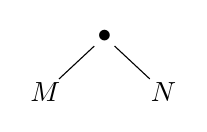
\begin{tikzpicture}[baseline=-3pt,level distance=7mm,
		every node/.style={inner sep=1pt}]
		\node {$\bullet$}
		child { node {$M$} }
		child { node {$N$} };
	\end{tikzpicture}
\]
This mapping is bijective between program terms (modulo $\alpha$-conversion) and
labeled elements of $\mathcal{C}$.

Pairs-expansions of combinators---for example the standard expansions of
$\mathrm{S}$ and $\mathrm{K}$ into $\lambda$-terms—produce larger trees but
remain within the Catalan family.  Thus the Catalan substrate is closed under
syntactic elaboration.

Operational semantics are likewise internal.  Both $\beta$-reduction and SKI
contraction replace subtrees with simpler subtrees while preserving the global
full-binary-tree form.  Each admissible reduction path therefore corresponds to
a trajectory within $\mathcal{C}$, and nondeterminism in reduction strategy
corresponds to branching structure within the Catalan tree itself.

This uniformity demonstrates that the Catalan substrate simultaneously captures:
\begin{enumerate}
	\item program syntax (binary application structure),
	\item program elaboration (via pairs-expansion or substitution), and
	\item program dynamics (via evaluation rewrites).
\end{enumerate}
Consequently, computation lives entirely within the Catalan family, justifying
its use as the structural substrate for the unified causal--computational model
developed in the main text.

\subsection{Illustrative Figures}

\begin{figure}[h]
	\centering
	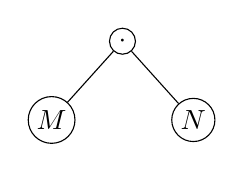
\begin{tikzpicture}[
		level distance=10mm,
		sibling distance=18mm,
		every node/.style={circle,draw,inner sep=1.5pt}
		]
		\node {$\cdot$}
			child { node {$M$} }
			child { node {$N$} };
	\end{tikzpicture}
	\caption{A binary application node representing the term $M\,N$.}
\end{figure}

\begin{figure}[h]
	\centering
	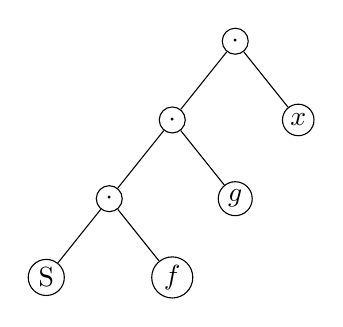
\begin{tikzpicture}[
		level distance=10mm,
		sibling distance=16mm,
		every node/.style={circle,draw,inner sep=1.5pt}
		]
		\node {$\cdot$}
			child {
				node {$\cdot$}
				child { node {$\cdot$} child { node {$\mathrm{S}$} } child { node {$f$} } }
				child { node {$g$} }
			}
			child { node {$x$} };
	\end{tikzpicture}
	\caption{Binary-tree representation of the term $\mathrm{S}\,f\,g\,x$.}
	\label{fig:Sfgx-binary-tree}
\end{figure}

\begin{figure}[h]
	\centering
	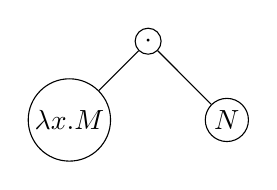
\begin{tikzpicture}[
		level distance=10mm,
		sibling distance=20mm,
		every node/.style={circle,draw,inner sep=1.5pt}
		]
		\node {$\cdot$}
			child { node {$\lambda x.M$} }
			child { node {$N$} };
	\end{tikzpicture}
	\qquad$\Longrightarrow$\qquad
	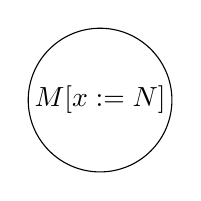
\begin{tikzpicture}[
		level distance=10mm,
		sibling distance=20mm,
		every node/.style={circle,draw,inner sep=1.5pt}
		]
		\node {$M[x:=N]$};
	\end{tikzpicture}
	\caption{$\beta$-reduction as a local rewrite inside the Catalan family.}
\end{figure}

\subsection{Pairs Expansion as Variable-Free S-Expressions}
\label{subsec:pairs-s-expressions}

A central observation motivating this work is that the pairs expansions of
combinators can be written as \emph{variable- and label-free} S-expressions,
exactly in the style of McCarthy's original Lisp notation \cite{McCarthy1960}.
In McCarthy's formulation, the core data structure is the cons-cell, written as
a parenthesized pair. Here we push this idea to an extreme: we erase all atom
labels and regard the program itself as a pure cons-tree, encoded only by
balanced parentheses.

Concretely, consider the binary application tree for the term
$\mathrm{S}\,f\,g\,x$ (as in Figure~\ref{fig:Sfgx-binary-tree}). Under the pairs
encoding used in our simulations, this same shape appears as the variable-free
S-expression
\[
	\texttt{(()(()(()())))}.
\]
This S-expression can also be understood as \emph{looking down into} the
underlying Catalan tree: the outer parentheses form the root frame, while each
\texttt{()} corresponds to a leaf. The corresponding unlabeled binary tree shape
is shown below.

\begin{center}
	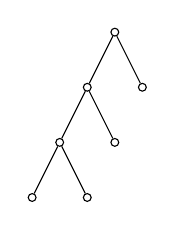
\begin{tikzpicture}[
		level 1/.style={level distance=7mm,sibling distance=7mm},
		level 2/.style={level distance=7mm,sibling distance=7mm},
		level 3/.style={level distance=7mm,sibling distance=7mm},
		every node/.style={circle,draw,inner sep=1pt,minimum size=2pt}
		]
		\node {}
			child { node {}
				child { node {}
					child { node {} }
					child { node {} }
				}
				child { node {} }
			}
			child { node {} };
	\end{tikzpicture}
\end{center}

Viewed from this perspective, the S-expression is simply the linear “parenthesis
trace” of this structure: each ``('' corresponds to descending into a cons-cell,
each ``)'' corresponds to returning toward the trunk, and the empty pairs
\texttt{()} mark the terminal leaves.

More generally, the pairs bijection

\begin{small}
\begin{verbatim}
n=0, c=1:  ()
n=1, c=1:  (()())
n=2, c=2:  (()(()())) ((()())())
n=3, c=5:  (()(()(()()))) (()((()())())) ((()())(()())) ((()(()()))()) (((()())())())
\end{verbatim}
\end{small}

enumerates exactly the same Catalan shapes that appear as Dyck paths

\begin{verbatim}
n=1, c=1:  ()
n=2, c=2:  (()) ()()
n=3, c=5:  ((())) (()()) (())() ()(()) ()()()
\end{verbatim}

but seen through a different projection. The Dyck words present the
one-dimensional ``height'' profile of the walk, making the Lorentzian scaling
limit and the breadth--depth structure of the light cone transparent. The pairs
S-expressions, by contrast, foreground the \emph{binary computational
structure}: they are precisely the unlabeled S-expression trees of a Lisp-like
language, with cons as the sole constructor.
\footnote{Here “projection’’ is not a literal mapping but a change of
	coordinates on the same Catalan object. The Dyck, binary-tree, and
	S-expression representations are all related by canonical bijections; each is
	a different parametrization of the same underlying Catalan shape.  Thus
switching from Dyck words to pairs S-expressions does not change the object
itself, only the coordinate system through which it is viewed.}

In this sense, Dyck words and pairs expansions are two complementary Catalan
bijections:

\begin{itemize}
	\item Dyck words: a one-dimensional time--breadth profile well adapted to
		continuum limits and Lorentzian geometry;
	\item pairs S-expressions: a fully binary application tree well adapted to
		combinatory computation.
\end{itemize}

Both encode the same Catalan shapes; one may view them as distinct ``Lorentz
frames'' on the same underlying combinatorial substrate. The pairs expansion can
thus be regarded as an additional invariant transform: it preserves the Catalan
class while re-expressing the same light-cone structure in purely computational
coordinates.

There is also an intrinsic handedness in this picture. Dyck words of a given
semilength $n$ are not symmetric under reversal of the walk; the distribution of
shapes across the tier reflects the left-to-right order in which parentheses are
added. This asymmetry is the combinatorial trace of the fundamental handedness
of applicative collapse in the pairs expansion: application is not commutative,
and the collapse rule is oriented. The sequential construction of the
S-expression tree makes this visible as a bias in how breadth is accumulated
relative to depth.

A further simplification arises when we observe that in the S-expression view,
explicit application nodes disappear entirely. Application is seen as a
\emph{property of the parentheses themselves}: a nested pair structure is
already an applicative program. From the standpoint of Schönfinkel's combinatory
logic \cite{Schoenfinkel1924}, where even the familiar $\mathrm{S}$ and
$\mathrm{K}$ can be reduced to a single sufficiently expressive combinator, one
may heuristically say that if a lone combinator $J$ acting on parentheses is
enough, then we can omit $J$ and work directly with the bare parentheses~$()$.
The Catalan substrate then becomes a \emph{combinator-free} calculus of pure
application.

Traditional functional calculi admit multiple evaluation strategies
(normal-order, applicative-order, call-by-need, etc.). The Catalan substrate
makes explicit a natural causal preorder on redex positions (ancestor order),
constraining dependencies between contractions. Collapse is local, and
contractions supported on disjoint subtrees commute
(Lemma~\ref{lem:causal-consistency}). Different evaluation strategies may then
be viewed as different linearizations of the residual freedom to schedule
causally independent contractions (Appendix~\ref{appendix:computational-foundations}).

\paragraph{Historical Perspective.}

The S-expression viewpoint connects the present framework to three classical
constructions.  First, McCarthy's original Lisp treats cons-pairs as the sole
data constructor, with atoms added as a separate syntactic category
\cite{McCarthy1960}. Here we invert the hierarchy: structure is primary, and
atoms---if present at all---arise as designated structural motifs.

Second, Church encodings demonstrate that data and control structures can be
represented entirely by higher-order functions; similarly, SKI combinatory logic
eliminates variables altogether. These developments show that symbolic reference
is not primitive but can be reconstructed from purely structural or operational
primitives.

Third, Gödel numbering treats syntax as arithmetic structure. The present
approach may be viewed as a ``Catalan numbering,'' where syntactic entities are
mapped to unlabeled binary trees. The Dyck, pairs, and binary-tree bijections
then provide multiple coordinate systems for the same structural universe. In
this sense, the Catalan substrate acts simultaneously as a computational
calculus and as a structural semantics for symbolic systems.

\subsection{Symbolic Representation in a Structure-Only Substrate}
\label{subsec:symbolic-representation}

In the Catalan substrate all information is structural: the only primitive
constructor is the cons-pair, and there are no atomic labels. This raises a
fundamental question: how can a system without atoms support symbols, naming, or
reference? The answer is that symbols arise not as primitives but as
\emph{structural motifs} that function as internal or external markers depending
on context. We distinguish two forms of symbolic representation.

\subsubsection{Internal Structural Symbols}

Within a closed Catalan machine, one may bootstrap symbolic reference by
designating particular tree shapes as internal ``names.'' A higher-level
self-referential mechanism (conceptually similar to a Y-like fixed-point
operator) can maintain a dictionary of such shapes, mapping them to programs,
behaviours, or combinator expansions. In this mode, names are themselves Catalan
objects, and symbolic reference arises entirely from geometry: identifying a
symbol is equivalent to matching a structural pattern. This yields a Lisp-like
environment without atomic identifiers, where all ``atoms'' are implemented as
canonical shapes in the tree.

\subsubsection{External Structural Symbols}

When interacting with external systems, the same structural motifs can serve as
\emph{extrinsic} symbols. Distinguished shapes may encode character codes,
vector-drawing glyphs, device signals, or other forms of I/O. This does not
modify the underlying calculus: it merely overlays a conventional interpretation
on structural patterns. The Catalan substrate remains atomless internally, while
external systems treat designated shapes as meaningful codes.

\subsubsection{Unified View: Symbols as Distinguished Motifs}

Both internal and external naming mechanisms exemplify a common principle: in a
structure-only universe, symbols are not primitive entities but \emph{designated
Catalan motifs}. A symbol is simply a tree pattern endowed—internally or
externally—with stable semantic interpretation. The substrate itself does not
distinguish between data and code, or between program and identifier; all such
distinctions emerge from the placement and recognition of specific structural
forms.

\begin{definition}[Structural Symbol]

	A \emph{structural symbol} is a finite Catalan tree $S$ together with an
	interpretation map $\iota$ assigning $S$ either (i) an internal computational
	meaning within the Catalan machine, or (ii) an external semantic meaning
	communicated to an outside system. The substrate recognizes $S$ only as a
	structure; all semantics flow from~$\iota$.

\end{definition}

\begin{remark}

	Although traditional programming languages begin with atoms and build
	structure on top of them, the Catalan substrate inverts this perspective:
	structure comes first, and atoms (if needed) are reintroduced later as
	structural patterns. From this viewpoint Lisp's cons-based representation, and
	even Schönfinkel's proposal of a single universal combinator, appear naturally
	as degenerate cases of a more general structure-first semantics.

\end{remark}


\subsection{Causal Admissibility of Redex Contraction}
\label{subsec:causal-admissibility}

We now formalize the sense in which evaluation order is fixed by causality
rather than chosen by convention.

\begin{definition}[Causal Preorder on Positions]
	Let $T$ be a full binary tree in the Catalan substrate, representing a program
	term. A \emph{position} in $T$ is a node address $p$ in the usual tree sense
	(e.g.\ a finite word over $\{L,R\}$ indicating left/right choices from the
	root). We write $p \prec q$ if the node at position $p$ lies on the unique
	path from the root to the node at position $q$. The reflexive, transitive
	closure of $\prec$ defines a preorder $\preceq$ on positions, which we call
	the \emph{causal preorder}.
\end{definition}

Intuitively, $p \preceq q$ means that the subtree at $q$ is causally downstream of the subtree at $p$: any change at $p$ may propagate to $q$ but not conversely.

\begin{definition}[Redex and Causal Admissibility]
	A \emph{redex} in $T$ is a position $p$ such that the subtree rooted at $p$
	matches the left-hand side of a reduction rule (e.g.\ a $\beta$-redex or an
	SKI contraction). Let $R(T)$ be the set of all redex positions in $T$.

	A redex at position $p \in R(T)$ is \emph{causally admissible} if there is no
	other redex $q \in R(T)$ with $q \prec p$. In other words, a redex is causally
	admissible if it is minimal in $R(T)$ with respect to the strict causal order.
\end{definition}

\begin{definition}[Causally Admissible Reduction Sequence]
	A finite or infinite sequence of trees
	\[
		T_0 \to T_1 \to T_2 \to \cdots
	\]
	is \emph{causally admissible} if, for each step $T_i \to T_{i+1}$, the
	contracted redex is causally admissible in $T_i$ in the above sense. A
	\emph{causal computation} is a causally admissible sequence starting from some
	initial tree $T_0$.
\end{definition}


\begin{lemma}[Commutation of disjoint reductions]
	\label{lem:causal-consistency}
	Let $T$ be a Catalan tree (full binary tree) and let $p,q\in R(T)$ be two redex
	positions that are \emph{incomparable} under the causal preorder $\preceq$
	(i.e.\ neither lies on the path from the root to the other). Let $T_p$ denote
	the result of contracting the redex at $p$, and similarly $T_q$.
	Then $q$ remains a redex position in $T_p$ and $p$ remains a redex position in
	$T_q$, and contracting both redexes yields the same tree regardless of order:
	\[
		(T_p)_q \;\equiv\; (T_q)_p.
	\]
	In particular, disjoint reductions form a commuting diamond as in
	Figure~\ref{fig:disjoint-subtrees}.
\end{lemma}

\begin{proof}[Proof Sketch]
	Since $p$ and $q$ lie in disjoint subtrees, contracting at $p$ rewrites only
	the subtree rooted at $p$ and leaves the subtree rooted at $q$ unchanged. Thus
	the redex at $q$ is unaffected (and remains at the same position), so it may
	still be contracted in $T_p$. Symmetrically, contracting at $q$ leaves the
	subtree at $p$ unchanged. Because the two rewrite steps act on disjoint parts
	of the tree, performing both contractions yields the same result regardless of
	order.
\end{proof}


\subsection{Evaluation Strategies as Coarse-Grainings of Causal Order}
\label{subsec:evaluation-strategies}

Traditional presentations of the $\lambda$-calculus distinguish several
evaluation strategies: normal-order, applicative-order, call-by-need, and many
others. These are usually defined syntactically (e.g.\ by specifying which redex
is chosen at each step), with confluence guaranteeing that they terminate in the
same normal form when one exists. In the Catalan substrate, however, causality
constrains redex selection more tightly.

\begin{definition}[Strategy-Compatible Causal Computation]
	Let $\mathcal{S}$ be a syntactic evaluation strategy (e.g.\ normal-order or
	applicative-order) which, given a term, selects one or more redex positions
	considered ``eligible'' at each step. A causal computation
	\[
		T_0 \to T_1 \to \cdots
	\]
	is \emph{compatible} with $\mathcal{S}$ if, at each step, the contracted redex
	is both causally admissible in $T_i$ and belongs to the set of redexes
	selected by $\mathcal{S}$ for the corresponding term.
\end{definition}

\begin{proposition}[Strategies as Coarse-Grainings of Causal Structure]
	\label{prop:strategies-coarse-graining}
	Let $T_0$ be an initial term, and suppose $\mathcal{S}$ is a standard
	evaluation strategy that is normalizing on $T_0$ (e.g.\ normal-order for a
	weakly normalizing term). Then:
	\begin{enumerate}
		\item Every $\mathcal{S}$-guided reduction sequence can be refined to a
			causally admissible computation by reordering only reductions that occur
			at redexes incomparable under the causal preorder.
		\item Conversely, every causally admissible computation from $T_0$ to normal
			form projects to an $\mathcal{S}$-valid history by forgetting the precise
			interleaving of causally independent reductions.
	\end{enumerate}
	In this sense, classical evaluation strategies are coarse-grainings of the
	underlying causal order: they differ only in how they resolve the residual
	freedom to permute causally independent redex contractions.
\end{proposition}

\begin{proof}[Proof Sketch]
	For (1), observe that any $\mathcal{S}$-guided sequence that temporarily
	contracts a non-minimal redex (with respect to $\preceq$) must do so in a
	context where all redexes on which it causally depends will eventually be
	contracted as well. By standard commuting-conversion arguments, we can reorder
	the sequence so that causally prior redexes are contracted first, without
	changing the final normal form. This reordering affects only redexes that lie
	in disjoint subtrees, i.e.\ are incomparable under $\preceq$.

	For (2), given a causally admissible computation, we can group together all
	contractions that $\mathcal{S}$ regards as taking place at the ``same'' redex
	position in the syntactic term, ignoring the precise ordering among
	contractions in disjoint subtrees. The resulting abstract history matches what
	$\mathcal{S}$ would produce, by confluence and the fact that $\mathcal{S}$ is
	normalizing on $T_0$. Thus $\mathcal{S}$ may be seen as a projection that
	forgets the fine-grained causal structure of independent collapses while
	preserving the global reduction behaviour.
	\end{proof}

	\bibliographystyle{plain}
	\begin{thebibliography}{99}

	\bibitem{addario-berry13}
	L.~Addario-Berry, L.~Devroye, and S.~Janson.
	\newblock Sub-Gaussian tail bounds for the width and height of conditioned
	Galton--Watson trees.
	\newblock {\em Annals of Probability}, 41(2):1074--1087, 2013.

	\bibitem{ambjorn01}
	J.~Ambj{\o}rn, J.~Jurkiewicz, and R.~Loll.
	\newblock Dynamically triangulating Lorentzian quantum gravity.
	\newblock {\em Nuclear Physics B}, 610:347--382, 2001.

	\bibitem{ambjorn12}
	J.~Ambj{\o}rn, A.~G{\"o}rlich, J.~Jurkiewicz, and R.~Loll.
	\newblock Nonperturbative quantum gravity.
	\newblock {\em Physics Reports}, 519:127--210, 2012.

	\bibitem{barendregt84}
	H.~P. Barendregt.
	\newblock {\em The Lambda Calculus: Its Syntax and Semantics}.
	\newblock North-Holland, 1984.

	\bibitem{bombelli87}
	L.~Bombelli, J.~Lee, D.~Meyer, and R.~D. Sorkin.
	\newblock Space-time as a causal set.
	\newblock {\em Physical Review Letters}, 59(5):521--524, 1987.

	\bibitem{church33}
	A.~Church.
	\newblock A set of postulates for the foundation of logic.
	\newblock {\em Annals of Mathematics}, 34:839--864, 1933.

	\bibitem{cover-thomas}
	T.~M. Cover and J.~A. Thomas.
	\newblock {\em Elements of Information Theory}.
	\newblock 2nd edition, John Wiley \& Sons, 2006.

	\bibitem{CurryFeys1958}
	H.~B. Curry and R.~Feys.
	\newblock {\em Combinatory Logic, Vol.~I}.
	\newblock North-Holland, 1958.

	\bibitem{curry58}
	H.~B. Curry.
	\newblock {\em Foundations of Mathematical Logic}.
	\newblock McGraw--Hill, 1958.

	\bibitem{feynman-hibbs65}
	R.~P. Feynman and A.~R. Hibbs.
	\newblock {\em Quantum Mechanics and Path Integrals}.
	\newblock McGraw--Hill, 1965. (Dover reprint, 2010).

	\bibitem{janson07}
	S.~Janson.
	\newblock Brownian excursion area, Wright's constants in graph enumeration, and
	other Brownian areas.
	\newblock {\em Probability Surveys}, 4:80--145, 2007.

	\bibitem{kac49}
	M.~Kac.
	\newblock On distributions of certain Wiener functionals.
	\newblock {\em Transactions of the American Mathematical Society},
	65(1):1--13, 1949.

	\bibitem{le-gall05}
	J.-F. Le~Gall.
	\newblock Random trees and applications.
	\newblock {\em Probability Surveys}, 2:245--311, 2005.

	\bibitem{McCarthy1960}
	J.~McCarthy.
	\newblock Recursive functions of symbolic expressions and their computation by
	machine, Part I.
	\newblock {\em Communications of the ACM}, 3(4):184--195, 1960.

	\bibitem{orus14}
	R.~Or\'us.
	\newblock A practical introduction to tensor networks: Matrix product states and
	projected entangled pair states.
	\newblock {\em Annals of Physics}, 349:117--158, 2014.

	\bibitem{rovelli04}
	C.~Rovelli.
	\newblock {\em Quantum Gravity}.
	\newblock Cambridge University Press, 2004.

	\bibitem{Schoenfinkel1924}
	M.~Sch{\"o}nfinkel.
	\newblock {\"U}ber die Bausteine der mathematischen Logik.
	\newblock {\em Mathematische Annalen}, 92:305--316, 1924.

	\bibitem{stanley-catalan}
	R.~P. Stanley.
	\newblock {\em Catalan Numbers}.
	\newblock Cambridge University Press, 2015.

\end{thebibliography}
\end{document}
